% Options for packages loaded elsewhere
\PassOptionsToPackage{unicode}{hyperref}
\PassOptionsToPackage{hyphens}{url}
\PassOptionsToPackage{dvipsnames,svgnames,x11names}{xcolor}
%
\documentclass[
  number,
  preprint,
  3p]{elsarticle}

\usepackage{amsmath,amssymb}
\usepackage{iftex}
\ifPDFTeX
  \usepackage[T1]{fontenc}
  \usepackage[utf8]{inputenc}
  \usepackage{textcomp} % provide euro and other symbols
\else % if luatex or xetex
  \usepackage{unicode-math}
  \defaultfontfeatures{Scale=MatchLowercase}
  \defaultfontfeatures[\rmfamily]{Ligatures=TeX,Scale=1}
\fi
\usepackage{lmodern}
\ifPDFTeX\else  
    % xetex/luatex font selection
\fi
% Use upquote if available, for straight quotes in verbatim environments
\IfFileExists{upquote.sty}{\usepackage{upquote}}{}
\IfFileExists{microtype.sty}{% use microtype if available
  \usepackage[]{microtype}
  \UseMicrotypeSet[protrusion]{basicmath} % disable protrusion for tt fonts
}{}
\makeatletter
\@ifundefined{KOMAClassName}{% if non-KOMA class
  \IfFileExists{parskip.sty}{%
    \usepackage{parskip}
  }{% else
    \setlength{\parindent}{0pt}
    \setlength{\parskip}{6pt plus 2pt minus 1pt}}
}{% if KOMA class
  \KOMAoptions{parskip=half}}
\makeatother
\usepackage{xcolor}
\setlength{\emergencystretch}{3em} % prevent overfull lines
\setcounter{secnumdepth}{5}
% Make \paragraph and \subparagraph free-standing
\ifx\paragraph\undefined\else
  \let\oldparagraph\paragraph
  \renewcommand{\paragraph}[1]{\oldparagraph{#1}\mbox{}}
\fi
\ifx\subparagraph\undefined\else
  \let\oldsubparagraph\subparagraph
  \renewcommand{\subparagraph}[1]{\oldsubparagraph{#1}\mbox{}}
\fi


\providecommand{\tightlist}{%
  \setlength{\itemsep}{0pt}\setlength{\parskip}{0pt}}\usepackage{longtable,booktabs,array}
\usepackage{calc} % for calculating minipage widths
% Correct order of tables after \paragraph or \subparagraph
\usepackage{etoolbox}
\makeatletter
\patchcmd\longtable{\par}{\if@noskipsec\mbox{}\fi\par}{}{}
\makeatother
% Allow footnotes in longtable head/foot
\IfFileExists{footnotehyper.sty}{\usepackage{footnotehyper}}{\usepackage{footnote}}
\makesavenoteenv{longtable}
\usepackage{graphicx}
\makeatletter
\def\maxwidth{\ifdim\Gin@nat@width>\linewidth\linewidth\else\Gin@nat@width\fi}
\def\maxheight{\ifdim\Gin@nat@height>\textheight\textheight\else\Gin@nat@height\fi}
\makeatother
% Scale images if necessary, so that they will not overflow the page
% margins by default, and it is still possible to overwrite the defaults
% using explicit options in \includegraphics[width, height, ...]{}
\setkeys{Gin}{width=\maxwidth,height=\maxheight,keepaspectratio}
% Set default figure placement to htbp
\makeatletter
\def\fps@figure{htbp}
\makeatother

\usepackage{booktabs}
\usepackage{longtable}
\usepackage{array}
\usepackage{multirow}
\usepackage{wrapfig}
\usepackage{float}
\usepackage{colortbl}
\usepackage{pdflscape}
\usepackage{tabu}
\usepackage{threeparttable}
\usepackage{threeparttablex}
\usepackage[normalem]{ulem}
\usepackage{makecell}
\usepackage{xcolor}
\usepackage{algorithm}
\usepackage{algpseudocode}
\makeatletter
\@ifpackageloaded{tcolorbox}{}{\usepackage[skins,breakable]{tcolorbox}}
\@ifpackageloaded{fontawesome5}{}{\usepackage{fontawesome5}}
\definecolor{quarto-callout-color}{HTML}{909090}
\definecolor{quarto-callout-note-color}{HTML}{0758E5}
\definecolor{quarto-callout-important-color}{HTML}{CC1914}
\definecolor{quarto-callout-warning-color}{HTML}{EB9113}
\definecolor{quarto-callout-tip-color}{HTML}{00A047}
\definecolor{quarto-callout-caution-color}{HTML}{FC5300}
\definecolor{quarto-callout-color-frame}{HTML}{acacac}
\definecolor{quarto-callout-note-color-frame}{HTML}{4582ec}
\definecolor{quarto-callout-important-color-frame}{HTML}{d9534f}
\definecolor{quarto-callout-warning-color-frame}{HTML}{f0ad4e}
\definecolor{quarto-callout-tip-color-frame}{HTML}{02b875}
\definecolor{quarto-callout-caution-color-frame}{HTML}{fd7e14}
\makeatother
\makeatletter
\@ifpackageloaded{caption}{}{\usepackage{caption}}
\AtBeginDocument{%
\ifdefined\contentsname
  \renewcommand*\contentsname{Table of contents}
\else
  \newcommand\contentsname{Table of contents}
\fi
\ifdefined\listfigurename
  \renewcommand*\listfigurename{List of Figures}
\else
  \newcommand\listfigurename{List of Figures}
\fi
\ifdefined\listtablename
  \renewcommand*\listtablename{List of Tables}
\else
  \newcommand\listtablename{List of Tables}
\fi
\ifdefined\figurename
  \renewcommand*\figurename{Figure}
\else
  \newcommand\figurename{Figure}
\fi
\ifdefined\tablename
  \renewcommand*\tablename{Table}
\else
  \newcommand\tablename{Table}
\fi
}
\@ifpackageloaded{float}{}{\usepackage{float}}
\floatstyle{ruled}
\@ifundefined{c@chapter}{\newfloat{codelisting}{h}{lop}}{\newfloat{codelisting}{h}{lop}[chapter]}
\floatname{codelisting}{Listing}
\newcommand*\listoflistings{\listof{codelisting}{List of Listings}}
\makeatother
\makeatletter
\makeatother
\makeatletter
\@ifpackageloaded{caption}{}{\usepackage{caption}}
\@ifpackageloaded{subcaption}{}{\usepackage{subcaption}}
\makeatother
\journal{Journal of Multivariate Analysis}
\ifLuaTeX
  \usepackage{selnolig}  % disable illegal ligatures
\fi
\usepackage[]{natbib}
\bibliographystyle{elsarticle-num-names}
\usepackage{bookmark}

\IfFileExists{xurl.sty}{\usepackage{xurl}}{} % add URL line breaks if available
\urlstyle{same} % disable monospaced font for URLs
\hypersetup{
  pdftitle={Studying the Performance of the Jellyfish Optimiser for the Application of Projection Pursuit},
  pdfauthor={Alice Anonymous; Bob Security; Cat Memes; Derek Zoolander},
  pdfkeywords={projection pursuit, optimization, jellyfish
optimiser, data visualisation, high-dimensional data},
  colorlinks=true,
  linkcolor={blue},
  filecolor={Maroon},
  citecolor={Blue},
  urlcolor={Blue},
  pdfcreator={LaTeX via pandoc}}

\setlength{\parindent}{6pt}
\begin{document}

\begin{frontmatter}
\title{Studying the Performance of the Jellyfish Optimiser for the
Application of Projection Pursuit}
\author[1]{Alice Anonymous%
\corref{cor1}%
}
 \ead{alice@example.com} 
\author[2]{Bob Security%
%
}
 \ead{bob@example.com} 
\author[2]{Cat Memes%
%
}
 \ead{cat@example.com} 
\author[]{Derek Zoolander%
%
}
 \ead{derek@example.com} 

\affiliation[1]{organization={Some Institute of Technology, Department
Name},addressline={Street Address},city={City},postcode={Postal
Code},postcodesep={}}
\affiliation[2]{organization={Another University, Department
Name},addressline={Street Address},city={City},postcode={Postal
Code},postcodesep={}}

\cortext[cor1]{Corresponding author}




        
\begin{abstract}
This is the abstract. Lorem ipsum dolor sit amet, consectetur adipiscing
elit. Vestibulum augue turpis, dictum non malesuada a, volutpat eget
velit. Nam placerat turpis purus, eu tristique ex tincidunt et. Mauris
sed augue eget turpis ultrices tincidunt. Sed et mi in leo porta
egestas. Aliquam non laoreet velit. Nunc quis ex vitae eros aliquet
auctor nec ac libero. Duis laoreet sapien eu mi luctus, in bibendum leo
molestie. Sed hendrerit diam diam, ac dapibus nisl volutpat vitae.
Aliquam bibendum varius libero, eu efficitur justo rutrum at. Sed at
tempus elit.
\end{abstract}





\begin{keyword}
    projection pursuit \sep optimization \sep jellyfish
optimiser \sep data visualisation \sep 
    high-dimensional data
\end{keyword}
\end{frontmatter}
    
\emph{Let's use British English (``American or British usage is
accepted, but not a mixture of these'')}

\section{Introduction {[}Nicolas and
Jessica{]}}\label{introduction-nicolas-and-jessica}

The artificial jellyfish search (JS) algorithm \citep{chou_novel_2021}
is a swarm-based metaheuristic optimisation algorithm inspired by the
search behaviour of jellyfish in the ocean. It is one of the newest
swarm intelligence algorithms \citep{rajwar_exhaustive_2023}, which was
shown to have stronger search ability and faster convergence with few
algorithmic parameters compared to classic optimization methods
\citep{chou_novel_2021}-\citep{chou_recent_2022}.

Effective optimisation is an important aspect of many methods employed
for visualising high-dimensional data (\(X\)). Here we are concerned
about computing informative linear projections of high-dimensional
(\(p\)) data using projection pursuit (PP) (\citet{kr69}, \citet{FT74}).
This involves optimising a function (e.g. \citet{hall1989polynomial},
\citet{cook1993projection}, \citet{lee2010projection},
\citet{Loperfido2018}, \citet{Loperfido2020}), called the projection
pursuit index (PPI), that defines what is interesting or informative in
a projection.

These PPI are defined on projections (\(XA\)), which means that there is
a constraint that needs to be considered when optimising. A projection
of data is defined by a \(p\times d\) orthonormal matrix \(A\), and this
imposes the constraint on the elements of \(A\), that columns need have
norm equal to 1 and the product of columns need to sum to zero.

\citet{cook1995grand} introduced the PP guided tour, which enabled
interactive visualisation of the optimisation in order to visually
explore high-dimensional data. It is implemented in the R \citep{R}
package \texttt{tourr} \citep{tourr}. The optimisation that is
implemented is fairly basic, and potential problems were highlighted by
\citet{RJ-2021-105}. Implementing better optimisation functionality is a
goal, but it needs to be kept in mind that the guided tour also has
places importance on watching the projected data as the optimisation
progresses.

Here we explore the potential for a jellyfish optimisation to be
integrated with the guided tour. Section~\ref{sec-background} explains
the optimisation that is used in the current the projection pursuit
guided tour. Section~\ref{sec-theory} provides more details on the
jellyfish optimiser and formalises several characteristics of projection
pursuit indexes that are help to measure optimisaer performance.
Section~\ref{sec-simulation} describes a simulation study on performance
of the jellyfish for several types of data and index functions.
Section~\ref{sec-conclusion} summarises the work and provides
suggestions for future directions.

\section{Projection pursuit, index functions and optimisation {[}Di and
Sherry{]}}\label{sec-background}

A tour on high-dimensional data is constructed by geodesically
interpolating between pairs of planes. Any plane is described by an
orthonormal basis, \(A_t\), where \(t\) represents time in the sequence.
The term ``geodesic'' refers to maintaining the orthonormality
constraint so that each view shown is correctly a projection of the
data. The PP guided tour operates by geodesically interpolating to
target planes (projections) which have high PP index values, as provided
by the optimiser. The geodesic interpolation means that the viewer sees
a continuous sequence of projections of the data, so they can watch
patterns of interest forming as the function is optimised. There are
five optimisation methods implemented in the \texttt{tourr} package:

\begin{itemize}
\tightlist
\item
  \texttt{search\_geodesic()}: provides a pseudo-derivative
  optimisation. It searches locally for the best direction, based on
  differencing the index values for very close projections. Then it
  follows the direction along the geodesic path between planes, stopping
  when the next index value fails to increase.
\item
  \texttt{search\_better()}: is a brute-force optimisation searching
  randomly for projections with higher index values.
\item
  \texttt{search\_better\_random()}: is essentially simulated annealing
  \citep{Bertsimas93} where the search space is reduced as the
  optimisation progresses.
\item
  \texttt{search\_posse()}: implements the algorithm described in
  \citet{posse95}.
\item
  \texttt{search\_polish()}: is a very localised search, to take tiny
  steps to get closer to the local maximum.
\end{itemize}

There are several PP index functions available: \texttt{holes()} and
\texttt{cmass()} \citep{cook1993projection}; \texttt{lda\_pp()}
\citep{lee2005projection}; \texttt{pda\_pp()} \citep{lee2010projection};
\texttt{dcor2d()} and \texttt{splines2d()} \citep{Grimm2016};
\texttt{norm\_bin()} and \texttt{norm\_kol()} \citep{huber85};
\texttt{slice\_index()} \citep{Laa:2020wkm}. Most are relatively simply
defined, for any projection dimension, and implemented because they are
relatively easy to optimise. A goal is to be able to incorporate more
complex PP indexes, for example based on scagnostics (\citet{scag},
\citet{WW08}).

An initial investigation of PP indexes, and the potential for
scagnostics is described in \citet{laa_using_2020}. To be useful here an
optimiser needs to be able to handle functions which are not very
smooth. In addition, because data structures might be relatively fine,
the optimiser needs to be able to find maxima that occur with a small
squint angle, that can only be seen from very close by. One last aspect
that is useful is for an optimiser to return local maxima in addition to
global because data can contain many different and interesting features.

\section{The jellyfish optimiser and properties of PP indexes {[}Nicolas
and Jessica{]}}\label{sec-theory}

The jellyfish optimiser (JSO) mimics the natural movements of jellyfish,
which include passive and active motions driven by ocean currents and
their swimming patterns, respectively. In the context of optimization,
these movements are abstracted to explore the search space in a way that
balances exploration (searching new areas) and exploitation (focusing on
promising areas). The algorithm aims to find the optimal solution by
adapting the jellyfish's behaviour to navigate towards the best solution
over iterations \citep{chou_novel_2021}.

To understand what the jellyfish optimizer is doing in the context of
Projection Pursuit, we first start with a current projection (the
starting point). Then, we evaluate this projection using an index
function, which tells us how good the current projection is. We then
move the projection in a direction determined by the `best jelly' and
random factors, influenced by how far along we are in the optimization
process (the trial \(i\) and \texttt{max.tries}). Occasionally, we might
explore completely new directions like a jellyfish might with ocean
currents. Then, we compare new potential projections to our current one.
If they're better, we adopt them; if not, we stick with our current
projection. This process continues and iteratively improves the
projection, until we reach the maximum number of trials.

\begin{tcolorbox}[enhanced jigsaw, arc=.35mm, titlerule=0mm, colframe=quarto-callout-note-color-frame, bottomtitle=1mm, opacitybacktitle=0.6, coltitle=black, colbacktitle=quarto-callout-note-color!10!white, rightrule=.15mm, opacityback=0, colback=white, toprule=.15mm, breakable, toptitle=1mm, left=2mm, bottomrule=.15mm, title={Algorithm: Jellyfish Optimizer Pseudo Code}, leftrule=.75mm]

\textbf{Input}: \texttt{current\_projections}, \texttt{index\_function},
\texttt{tries}, \texttt{max\_tries}

\textbf{Output}: \texttt{optimized\_projection}

\textbf{Initialize} \texttt{best\_jelly} as the projection with the best
index value from \texttt{current\_projections}, and
\texttt{current\_index} as the array of index values for each projection
in \texttt{current\_projections}

\textbf{for} each try in 1 to max\_tries \textbf{do}

\begin{quote}
Calculate \(c_t\) based on the current try and max\_tries
\end{quote}

\begin{quote}
\textbf{if} \(c_t\) is greater than or equal to \(0.5\) \textbf{then}

\begin{quote}
Define trend based on the best jelly and current projections
\end{quote}

\begin{quote}
Update each projection towards the trend using a random factor and
orthonormalisation
\end{quote}

\textbf{else}

\begin{quote}
\textbf{if} a random number is greater than \(1 - c_t\) \textbf{then}

\begin{quote}
Slightly adjust each projection with a small random factor (Type A
passive)
\end{quote}

\textbf{else}

\begin{quote}
For each projection, compare with a random jelly and adjust towards or
away from it (Type B active)
\end{quote}
\end{quote}

Update the orientation of each projection to maintain consistency

Evaluate the new projections using the index function
\end{quote}

\begin{quote}
\textbf{if} any new projection is worse than the current, revert to the
\texttt{current\_projection} for that case

\begin{quote}
Determine the projection with the best index value as the new
best\_jelly
\end{quote}
\end{quote}

\begin{quote}
\textbf{if} the try is the last one, print the final best projection and
\textbf{exit}
\end{quote}

\textbf{return} the set of projections with the updated best\_jelly as
the optimized\_projection

\end{tcolorbox}

The JSO implementation involves several key parameters that control its
search process in optimization problems. These parameters are designed
to guide the exploration and exploitation phases of the algorithm. While
the specific implementation details can vary depending on the version of
the algorithm or its application, we focus on two main parameters that
are most relevant to our application: the number of jellyfish and drift.

\citet{laa_using_2020} has proposed five criteria for assessing
projection pursuit indexes (smoothness, squintability, flexibility,
rotation invariance, and speed). Since not all the properties affects
the execution of the optimisation, here we consider the three relevant
properties (smoothness, squintability, and speed), and propose three
metrics to evaluate these three properties.

\subsection{Smoothness}\label{sec-smoothness}

If we evaluate the index function at some random points (like the random
initialization of the jellyfish optimizer), then we can interpret these
random index values as a random field, indexed by a space parameter: the
random projection angle. This analogy suggests to use this random
training sample to fit a spatial model, a simple one being a (spatial)
Gaussian process.

How can we define a measure of smoothness from this? The distribution of
a Gaussian process is fully determined by its mean function and
covariance function. The way the covariance function is defined is where
smoothness comes into play: if an index is very smooth, then two close
projection angles should produce close index values (strong
correlation); by contrast, if an index is not smooth, then two close
projection angles might give very different index values (fast decay of
correlations with respect to distance between angles).

Popular covariance functions are parametric positive semi-definite
functions, some of which have a parameter to capture the smoothness of
the Gaussian field. In particular, consider the Matérn class of
covariance functions, defined by

\[
K(u):=\frac{(\sqrt{2\nu}u)^{\nu}}{\Gamma(\nu)2^{\nu-1}}\mathcal{K}_{\nu}(\sqrt{2\nu}u)
\]

where \(\nu>0\) is the smoothness parameter and where
\(\mathcal{K}_\nu\) is the modified Bessel function. The Matérn
covariance function can be expressed analytically when \(\nu\) is a
half-integer, the most popular values in the literature being \(1/2\),
\(3/2\) and \(5/2\) . The parameter \(\nu\), called smoothness
parameter, controls the decay of the covariance function. As such, it is
an appropriate measure of smoothness of a random field.

In our context, we suggest to use this parameter as a measure of the
smoothness of the index function by fitting a Gaussian process prior
with Matérn covariance on a dataset generated by random evaluations of
the index function, as in the initial stage of the jellyfish random
search. There exist several R packages, such as GpGp or ExaGeoStatR, to
fit the hyperparameters of a GP covariance function on data. In this
project, we make use of the GpGp package.

The fitted value \(\nu>0\) can be interpreted as follows: the higher
\(\nu\), the smoother the index function.

\subsection{Squintability}\label{sec-squintability}

From the literature, it is commonly understood that a large squint angle
implies that the objective function value is close to optimal even when
we are not very close to the perfect view to see the structure. A small
squint angle means that index function value improves substantially only
when we are very close to the perfect view. As such, low squintability
implies rapid improvement in the index value when near the perfect view.

In this study, we propose two metrics to capture the notion of
squintability.

{[}We generate random points that is beyond 1.5 projection distance and
interpolate. Then we fit a kernel or use nonlinear least squares.{]}

First, parametric model.

{[}Nicolas's pdf{]}

Second, we consider the product of the largest absolute magnitude of
rate of change of \(f\) and the corresponding projection angle as a
second measure of squintability. Since \(f\) is decreasing, the rate of
change of \(f\) is negative and thus \(|\underset{x}{\min} f('x)|\)
gives the absolute magnitude of the most negative rate of change.

{[}Nicolas's pdf{]}

To the best of our knowledge, this is the first attempt to measure the
notion of squintability.

\subsection{Speed}\label{speed}

The speed of optimizing an index function can be calculated/measured
using the computational complexity (in big O notation, with respect to
the sample size) of computing the index function.

\section{Visualisation of jellyfish
optimiser}\label{visualisation-of-jellyfish-optimiser}

Information of the jellyfish optimiser is available in a tabular format
and below is an example data collected from finding the sine-wave
structure in 6D data using a distance correlation index
(\texttt{docr2d\_2}):

\begin{verbatim}
Rows: 10
Columns: 13
$ idx_f     <chr> "dcor2d_2", "dcor2d_2", "dcor2d_2", "dcor2d_2", "dcor2d_2", ~
$ d         <dbl> 6, 6, 6, 6, 6, 6, 6, 6, 6, 6
$ n_jellies <dbl> 20, 20, 20, 20, 20, 20, 20, 20, 20, 20
$ max_tries <dbl> 50, 50, 50, 50, 50, 50, 50, 50, 50, 50
$ sim       <int> 1, 1, 1, 1, 1, 1, 1, 1, 1, 1
$ seed      <int> 3462, 3462, 3462, 3462, 3462, 3462, 3462, 3462, 3462, 3462
$ basis     <list> <<matrix[6 x 2]>>, <<matrix[6 x 2]>>, <<matrix[6 x 2]>>, <<m~
$ index_val <dbl> 0.0247212373, 0.0033938502, 0.0463398915, 0.0486230801, -0.0~
$ info      <chr> "initiation", "initiation", "initiation", "initiation", "ini~
$ method    <chr> "search_jellyfish", "search_jellyfish", "search_jellyfish", ~
$ tries     <dbl> 1, 1, 1, 1, 1, 1, 1, 1, 1, 1
$ loop      <dbl> 1, 2, 3, 4, 5, 6, 7, 8, 9, 10
$ time      <drtn> 35.46031 secs, 35.46031 secs, 35.46031 secs, 35.46031 secs, ~
\end{verbatim}

Information recorded can be categorised into the following categories:

\begin{itemize}
\tightlist
\item
  projection pursuit variables: the index function used
  (\texttt{idx\_f}), the data dimension (\texttt{d})
\item
  jellyfish optimiser parameters: the number of jellies
  (\texttt{n\_jellies}), the maximum number of tries
  (\texttt{max\_tries})
\item
  simulation variables: the simulation number (\texttt{sim}), the seed
  used (\texttt{seed})
\item
  optimisation variables: the projection basis in a matrix format
  (\texttt{basis}), the index value (\texttt{index\_val}), a description
  of the status - one of ``initiation'', ``current\_best'', and
  ``jellyfish\_update'' (\texttt{info}), current iteration ID
  (\texttt{tries}), current jelly ID (\texttt{loop}), and the time taken
  to find the optimum (\texttt{time}).
\end{itemize}

The basis column records every basis \emph{visited} by the jellyfish
optimiser prior to comparing with the current basis. In each iteration,
if the index value of a visited basis is smaller than that of the
current one, the jellyfish optimiser will retain the current basis for
the next iteration, while still documenting the visited basis.

Numerical information to compute:

\begin{itemize}
\tightlist
\item
  angular distance between the projection basis and the theoretical best
  basis,
\item
  the proportion of simulation that found the optimal basis,
\item
  the proportion of jellies, within each simulation, that found the
  optimal basis,
\end{itemize}

Visualisation to inspect:

\begin{itemize}
\tightlist
\item
  inspect the basis visited by each jellyfish in the reduced PCA space,
\item
  inspect the final 2D projections reached by each jellyfish,
\item
  plot the index value against the angular distance between the
  projection basis and the theoretical best basis
\end{itemize}

Plotting the basis in the space and the projected data can help to
understand 1) whether each simulation finds the same optimum or some
simulations find local optima; and 2) whether the index function used
can detect the structure in the data and the projection contains the
structure of interest.

The visualisations above can be faceted by the projection pursuit
variables and jellyfish optimiser parameters to compare the performance
of different indexes to detect the same structure and how the jellyfish
optimiser parameters affect the optimisation process.

{[}example plots{]}

\begin{figure}[H]

{\centering 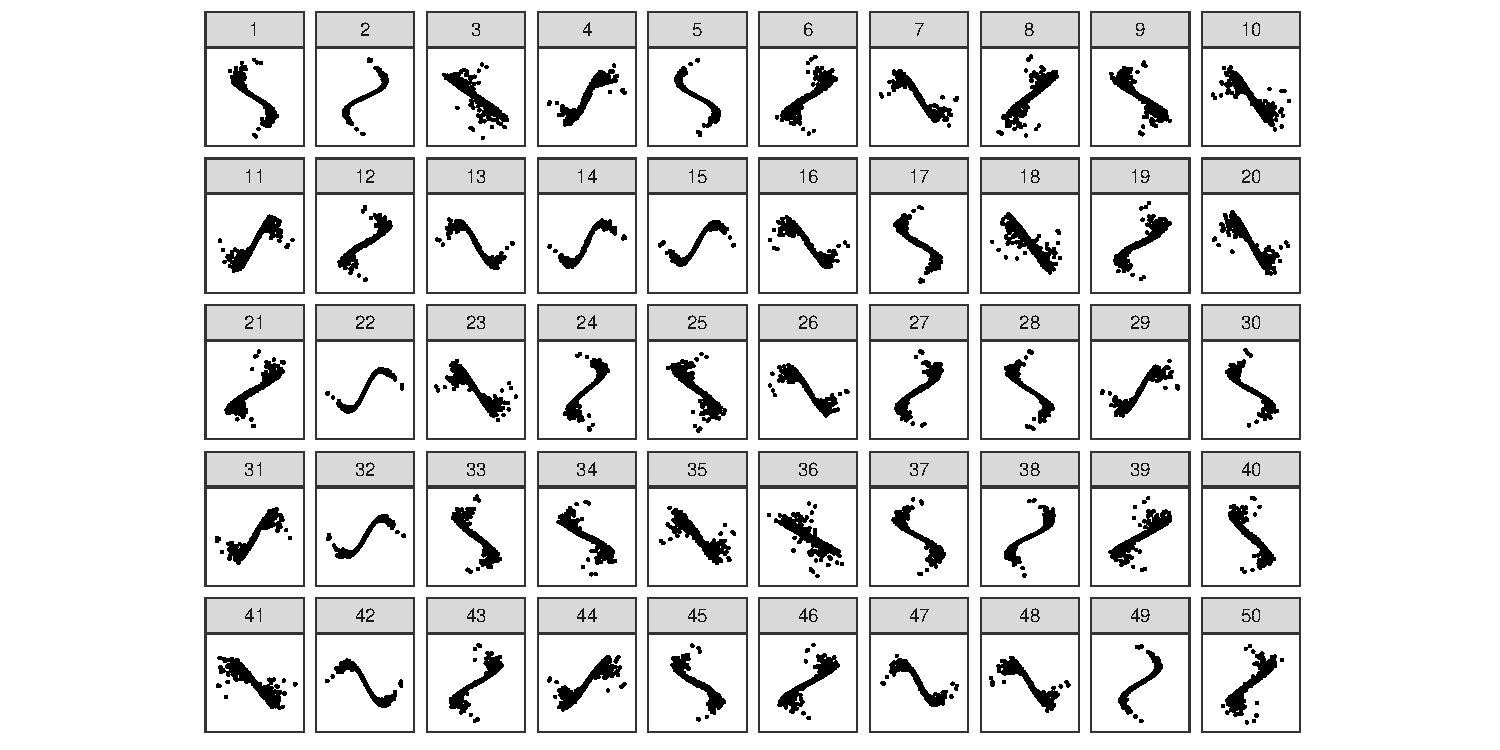
\includegraphics{optim_files/figure-pdf/unnamed-chunk-4-1.pdf}

}

\caption{sdfjsflk}

\end{figure}%

\section{Application {[}Di and Sherry{]}}\label{sec-simulation}

The jellyfish optimiser has been implemented in the tourr package
\citep{wickham_tourr_2011} and we will use the diagnostic plots proposed
in the ferrn package \citep{RJ-2021-105} to visualise the optimisation
process.

\subsection{Performance of the jellyfish optimiser in high-dimensional
pipe-finding
problems}\label{performance-of-the-jellyfish-optimiser-in-high-dimensional-pipe-finding-problems}

{[}unfinished{]}

The aim of this example is to investigate the performance of jellyfish
optimisers in high-dimensional problems.

The projection pursuit problem is to find the pipe shape, investigated
in \citet{laa_using_2020}, using the holes index in 6/8/10/12-D data.
For each case, 50 simulations are conducted for each combination of
jellyfish hyper-parameter: \texttt{n\_jellies\ =\ 20/50/100} and
\texttt{max\_tries\ =\ 50/100}. The performance of the jellyfish
optimiser is also compared with an existing opitmiser: the search better
opitmiser with \texttt{max.tries\ =\ 1000}.

Figure~\ref{fig-proportion} presents the proportion of jellyfishes that
finds the index value close to (absolute value less than 0.05) the best
index value found at each \texttt{max\_tries}/\texttt{n\_jellies}
combination at \(d = 6/8/10/12\) data dimension. As the number of
jellies and maximum tries increase, the proportion of jellyfishes that
find the optimal projection increases. This suggests for higher
dimensional problems (\(d = 8/10/12\)), an \texttt{n\_jellies\ =\ 100}
and \texttt{max\_tries\ =\ 100} is necessary for at least half of the
jellyfish optimiser to find the optimal projection.

Figure~\ref{fig-proj} presents the final projection found across the 50
simulations at each 10th quantile between the jellyfish and search
better optimiser (\texttt{n\_jellies\ =\ 100},
\texttt{max\_tries\ =\ 100} is used for the jellyfish optimiser). While
the jellyfish optimiser may not always find the optimal projection in
the worse case scenarios, especially as the dimension increases, it
tends to find higher index values and crisper pipe shapes than the
search better optimiser at each quantile across all the four data
dimensions.

\begin{figure}

\centering{

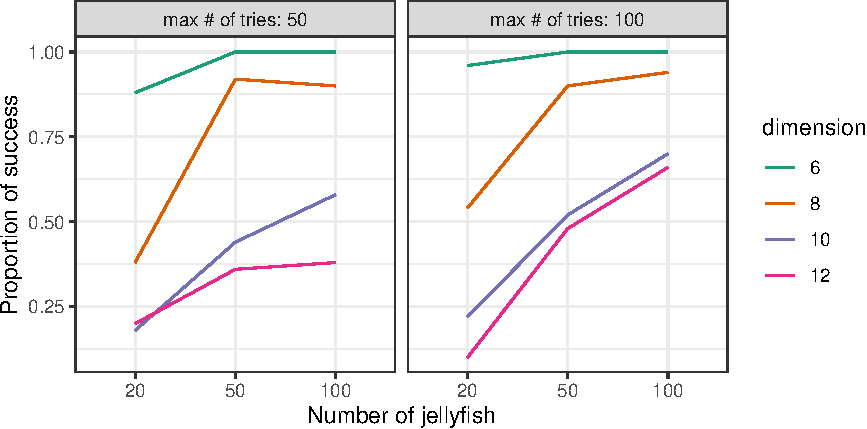
\includegraphics{optim_files/figure-pdf/fig-proportion-1.pdf}

}

\caption{\label{fig-proportion}Proportion of jellyfishes reaches close
to the optimal index value in the pipe-finding problem. As the dimension
goes up, the numer/ proportion of jellyfishes that reach the optimal
index value decreases. Increasing the jellyfish hyperparameters
(\texttt{n\_jellies} and \texttt{max\_tries}) help to improve the
proportion.}

\end{figure}%

\begin{figure}

\centering{

\includegraphics{optim_files/figure-pdf/fig-proj-1.pdf}

}

\caption{\label{fig-proj}Projections found by the jellyfish and search
better optimiser at each 10th quantile across 50 simulations. The holes
index is used to find the target pipe shape in the 6/8/10/12D space. An
\texttt{n\_jellies\ =\ 100} and \texttt{max\_tries\ =\ 100} are used for
the jellyfish optimiser and \texttt{max.tries\ =\ 1000} is used for the
search better optimiser.}

\end{figure}%

\subsection{Connecting optimisation success with its properties and
jellyfish
parameters}\label{connecting-optimisation-success-with-its-properties-and-jellyfish-parameters}

The optimisation properties (smoothness, squintability, and speed)
proposed in the Section~\ref{sec-theory} provide numerical measures to
characterise the difficulty of the optimisation for a given projection
pursuit problem. This example investigates how these measures, combined
with the jellyfish parameters, affect the success of the jellyfish
optimisers and how they can guide the decisions made in hyperparameter
tuning with the jellyfish optimiser. Simulations are conducted with
different jellyfish optimisers to obtain the proportion of successful
optimisation across a collection of scenarios, for which smoothness,
squintability, and speed are calculated. A generalised linear model is
used to link the proportion of success rate with the jellyfish
parameters and the optimisation properties.

In addition to the pipe-finding problem, also investigated is the
sine-wave finding problem in 6D and 8D spaces with six indices
considered: \texttt{dcor2d\_2}, \texttt{loess2d}, \texttt{MIC},
\texttt{TIC}, \texttt{spline}, and \texttt{stringy}. Combining with
different jellyfish optimiser parameters (\texttt{n\_jellies} and
\texttt{max\_tries}), a total of 52 cases is produced, comprising of 24
pipe-finding cases and 28 sine-wave finding cases. For each case, the
jellyfish optimiser is run fifty (50) times and summary statistics are
calculated on the best index value found across all 50 runs and the
proportion of runs that find a close (with a difference less than 0.05)
best index value (\texttt{P\_J\_hat}).

Smoothness and squintability are computed for each case, following the
procedures outlined in Section~\ref{sec-smoothness} and
Section~\ref{sec-squintability}. To calculate smoothness, three hundred
random bases are simulated. Index values and projection distance to the
optimal basis are calculated for each basis to fit a Gaussian process
model. For squintability, fifty random bases are sampled and
interpolated to the optimal basis with a step size of 0.005. The
interpolated bases are first binned with a bin width of 0.005 to average
the index values before feeding into a 4-parameter scaled logistic
function, estimated by non-linear least square, to obtain the
squintability measure.

Table~\ref{tbl-smoothness-squintability} presents the parameters
estimated for each case from the Gaussian process (variance, range,
smooth, and nugget) for smoothness and the scaled logistic function
(theta1 to theta4, and squint) for squintability. The column ``smooth''
and ``squint'' are used as the smoothness and squintability measure. The
low squint value of MIC and TIC index is due to its convex shape of the
index value against the projection distance, as shown in
Figure~\ref{fig-idx-proj-dist}. Comparing to other concave shapes, the
maximum first derivative happens at a smaller projection distance
(\(\theta2\)), requiring the optimiser to get closer to the optimal to
see a significant change in the index value, hence a small squintability
measure. {[}TODO: the stringy squintability doens't make sense{]}

Table~\ref{tbl-mod-data} presents the processed data for modelling after
augmenting the jellyfish parameters (\texttt{n\_jellies} and
\texttt{max\_tries}) and the average time spent on each run
(\texttt{time}) for each case. A generalised linear model is fitted with
a binomial family and a logit link function to the data to investigate
the relationship between the proportion of jellyfish success and
jellyfish parameters and the optimisation properties. Pre-processing of
the data include 1) scale the jellyfish parameters (\texttt{n\_jellies}
and \texttt{max\_tries}) by 10 for interpretation, and 2) create a
binary variable \texttt{long\_time} to flag the cases with average time
spent on each run greater than 30 seconds. Table~\ref{tbl-mod-output}
presents the model output with the estimated coefficients. The model
suggests a positive relationship between the proportion of jellyfish
success and the jellyfish parameters, \texttt{n\_jellies} and
\texttt{max\_tries}, optimisation property parameter,
\texttt{smoothness} and \texttt{squintability}, and a negative
relationship with the average time spent on each run
(\texttt{long\_time}) and the data dimension (\texttt{d}). The variable
\texttt{squintability} and \texttt{d} are significant, suggesting their
importance over jellyfish parameters to the success of the optimisation.

\begingroup\fontsize{7}{9}\selectfont

\begin{longtable}[t]{|>{}ll>{}r|rrr>{}r|rrrr>{}r|}

\caption{\label{tbl-smoothness-squintability}Parameters estimated from
the Gaussian process (including variance, range, smoothness, and nugget)
and scaled logistic function (theta1 to theta4) for the pipe-finding and
sine-wave finding problems. The squint column is calculated as
\(\frac{\theta1 \theta2 \theta3}{4}\), as described in
Section~\ref{sec-squintability}. The ``smooth'' and ``squint'' column
represent the smoothness and squintability measures.}

\tabularnewline

\toprule
shape & index & d & variance & range & smooth & nugget & theta1 & theta2 & theta3 & theta4 & squint\\
\midrule
pipe & holes & 6 & 0.002 & 0.408 & 2.364 & 0.212 & 1.001 & 0.860 & 3.368 & 0.823 & 0.725\\
pipe & holes & 8 & 0.000 & 0.259 & 2.373 & 0.613 & 1.001 & 0.869 & 3.264 & 0.811 & 0.710\\
pipe & holes & 10 & 0.000 & 0.144 & 2.317 & 1.831 & 1.000 & 0.885 & 3.151 & 0.806 & 0.697\\
pipe & holes & 12 & 0.000 & 0.254 & 2.173 & 0.879 & 1.000 & 0.878 & 3.345 & 0.806 & 0.734\\
sine & MIC & 6 & 0.016 & 0.100 & 2.394 & 0.087 & 0.894 & 0.571 & 1.623 & -0.024 & 0.207\\
\addlinespace
sine & MIC & 8 & 0.016 & 0.100 & 2.394 & 0.087 & 0.932 & 0.328 & 1.314 & -0.030 & 0.100\\
sine & TIC & 6 & 0.124 & 0.104 & 2.471 & 0.086 & 0.951 & 0.536 & 1.719 & -0.025 & 0.219\\
sine & TIC & 8 & 0.124 & 0.104 & 2.471 & 0.086 & 0.945 & 0.564 & 1.723 & -0.027 & 0.230\\
sine & dcor2d\_2 & 6 & 0.034 & 0.167 & 2.663 & 0.114 & 0.954 & 1.039 & 2.742 & -0.019 & 0.679\\
sine & loess2d & 6 & 0.083 & 0.307 & 2.194 & 0.292 & 1.016 & 1.039 & 2.648 & 0.080 & 0.699\\
\addlinespace
sine & splines2d & 6 & 0.040 & 0.189 & 2.606 & 0.104 & 1.014 & 1.051 & 2.730 & -0.009 & 0.727\\
sine & stringy & 6 & 0.000 & 1173.035 & 1.031 & 17608.047 & 1.011 & 0.011 & 254.734 & 0.727 & 0.711\\
\bottomrule

\end{longtable}

\endgroup{}

\begin{figure}

\centering{

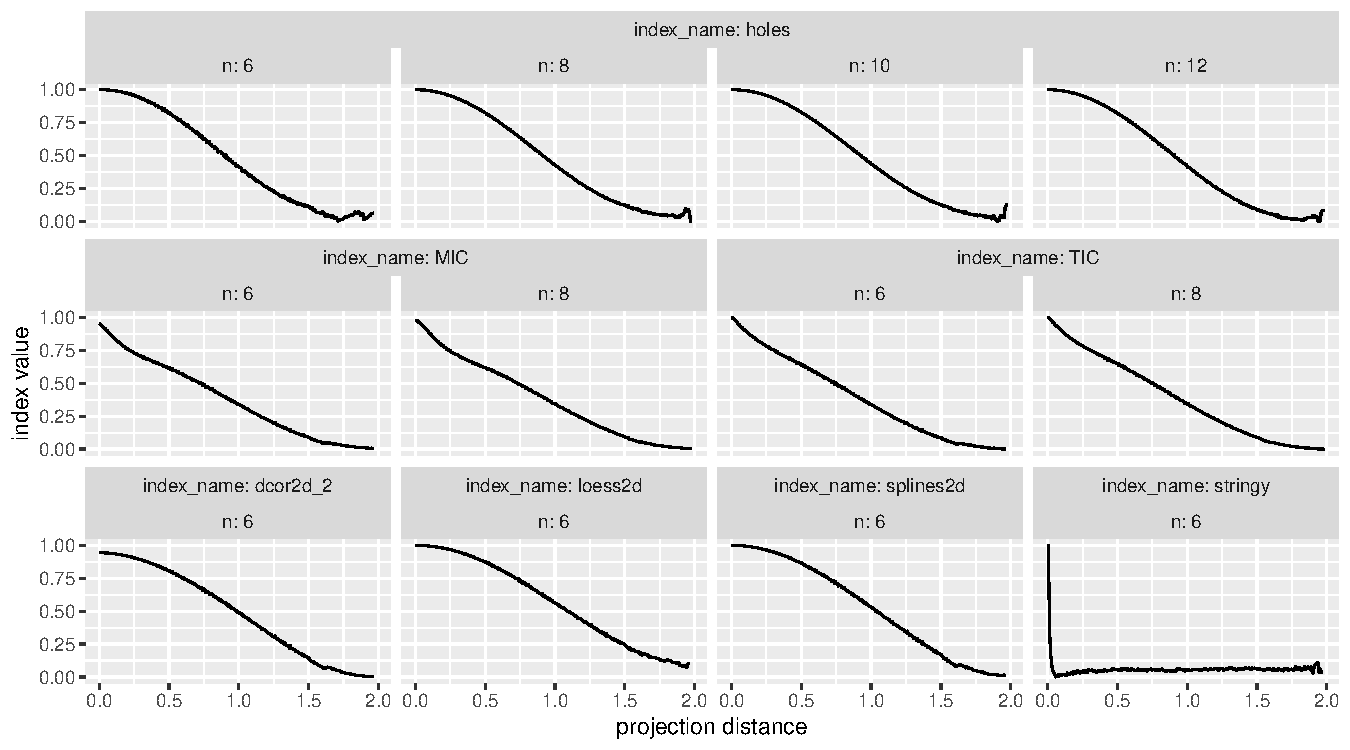
\includegraphics{optim_files/figure-pdf/fig-idx-proj-dist-1.pdf}

}

\caption{\label{fig-idx-proj-dist}Index values against projection
distance for the 12 pipe/sine-wave finding problem after the binning
procedure during the estimation of the squintability measure. The index
value is averaged at each bin width of 0.005 and the \texttt{TIC} index
is scaled to 0-1 for comparison. When finding the sine-wave structure
using the \texttt{MIC} and \texttt{TIC} index, a convex curved is
observed, as opposed to the pipe-finding problem or the sine-wave
finding problem with the \texttt{dcor2d\_2}, \texttt{loess2d}, and
\texttt{splines2d} index. When finding the sine-wave with the stringy
index, the index shows an instantaneous jump to the optimum when close
to the best basis.}

\end{figure}%

\begin{longtable}[]{@{}
  >{\raggedright\arraybackslash}p{(\columnwidth - 14\tabcolsep) * \real{0.0811}}
  >{\raggedleft\arraybackslash}p{(\columnwidth - 14\tabcolsep) * \real{0.0405}}
  >{\raggedleft\arraybackslash}p{(\columnwidth - 14\tabcolsep) * \real{0.1486}}
  >{\raggedleft\arraybackslash}p{(\columnwidth - 14\tabcolsep) * \real{0.1892}}
  >{\raggedleft\arraybackslash}p{(\columnwidth - 14\tabcolsep) * \real{0.1351}}
  >{\raggedleft\arraybackslash}p{(\columnwidth - 14\tabcolsep) * \real{0.1351}}
  >{\raggedleft\arraybackslash}p{(\columnwidth - 14\tabcolsep) * \real{0.1081}}
  >{\raggedright\arraybackslash}p{(\columnwidth - 14\tabcolsep) * \real{0.1622}}@{}}

\caption{\label{tbl-mod-data}The first few rows of the datasets
processed for modelling. The smoothness and squintability variable are
uniquely characterised by the index function used and the data
dimension, and thus do not vary across \texttt{n\_jellies} and
\texttt{max\_tries}. The variable \texttt{P\_J\_hat}, and time are
calculated at each observation.}

\tabularnewline

\toprule\noalign{}
\begin{minipage}[b]{\linewidth}\raggedright
index
\end{minipage} & \begin{minipage}[b]{\linewidth}\raggedleft
d
\end{minipage} & \begin{minipage}[b]{\linewidth}\raggedleft
smoothness
\end{minipage} & \begin{minipage}[b]{\linewidth}\raggedleft
squintability
\end{minipage} & \begin{minipage}[b]{\linewidth}\raggedleft
n\_jellies
\end{minipage} & \begin{minipage}[b]{\linewidth}\raggedleft
max\_tries
\end{minipage} & \begin{minipage}[b]{\linewidth}\raggedleft
P\_J\_hat
\end{minipage} & \begin{minipage}[b]{\linewidth}\raggedright
time
\end{minipage} \\
\midrule\noalign{}
\endhead
\bottomrule\noalign{}
\endlastfoot
MIC & 6 & 2.394 & 0.207 & 20 & 50 & 0.12 & 2.479 secs \\
MIC & 6 & 2.394 & 0.207 & 20 & 100 & 0.24 & 8.950 secs \\
MIC & 6 & 2.394 & 0.207 & 50 & 50 & 0.52 & 5.651 secs \\
MIC & 6 & 2.394 & 0.207 & 50 & 100 & 0.64 & 13.223 secs \\
MIC & 6 & 2.394 & 0.207 & 100 & 50 & 0.76 & 19.453 secs \\
MIC & 8 & 2.394 & 0.100 & 20 & 50 & 0.08 & 2.566 secs \\
MIC & 8 & 2.394 & 0.100 & 20 & 100 & 0.08 & 4.960 secs \\

\end{longtable}

\begin{longtable}[t]{|>{}lrrr>{}r|}

\caption{\label{tbl-mod-output}Model estimates of proportion of
jellyfish success (\texttt{P\_J\_hat}) on optimisation properties
(\texttt{smoothness}, \texttt{squintability}, and \texttt{d}) and
jellyfish parameters (\texttt{long\_time}, \texttt{n\_jellies}, and
\texttt{max\_tries}) from the generalised linear model with a binomial
family and a logit link function. The variable \texttt{long\_time} is
derived to flag the cases with average time spent on each run greater
than 30 seconds and the variable \texttt{n\_jellies} and
\texttt{max\_tries} are scaled by 10 for interpretation.}

\tabularnewline

\toprule
term & estimate & std.error & statistic & p.value\\
\midrule
intercept & -4.672 & 4.512 & -1.036 & 0.300\\
smoothness & 1.604 & 1.530 & 1.048 & 0.294\\
squintability & 7.062 & 2.210 & 3.195 & 0.001\\
d & -0.595 & 0.260 & -2.289 & 0.022\\
long\_time & -0.851 & 1.348 & -0.632 & 0.528\\
\addlinespace
n\_jellies & 0.230 & 0.131 & 1.754 & 0.080\\
max\_tries & 0.107 & 0.153 & 0.700 & 0.484\\
\bottomrule

\end{longtable}

\section{Conclusion {[}Di and Sherry{]}}\label{sec-conclusion}


\renewcommand\refname{References}
  \bibliography{bibliography.bib}


\end{document}
